\documentclass[bare_jrnl_transmag]{subfiles}
\begin{document}

\subsection{Kalman Filter Performance}
The performance of the Kalman filter was validated by plotting the output of the filter against the ground truth position of the drone in the world frame. The ground truth position was parsed from the dataset, and the Kalman filter was run on the raw sensor data, also parsed from the dataset. Using Matplotlib, both of these results were plotted on a 3D graph, with the x, y and z axes representing the world frame.

\begin{figure}[H]
    \centering
    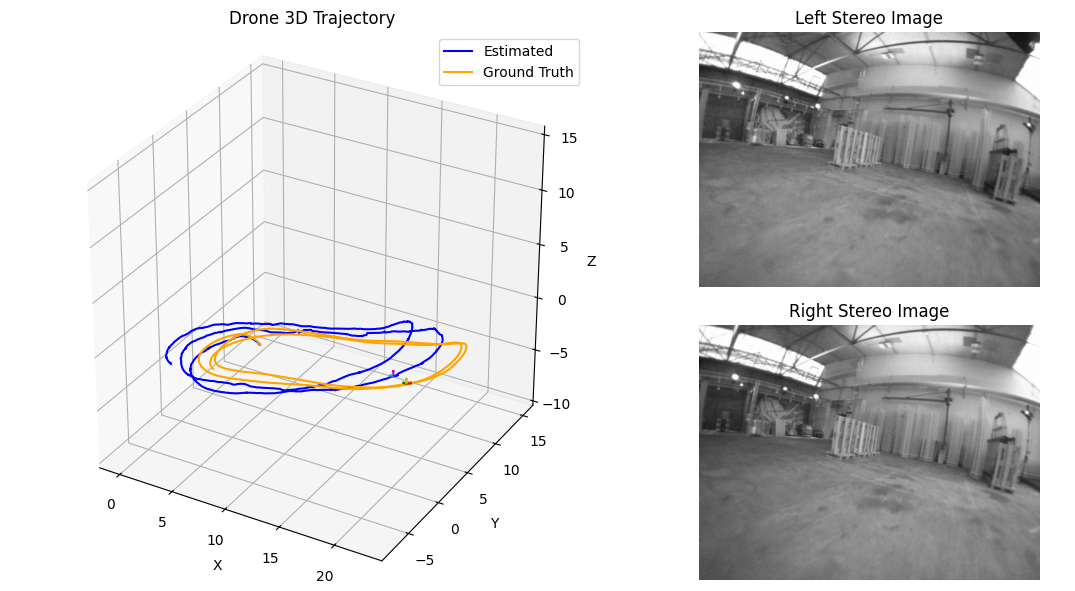
\includegraphics[width=0.8\linewidth]{figures/kf_results.png}
    \caption{Kalman filter results on testing set with tracks from both estimated and ground truth performance.}
    \label{fig:kalman_results_test_set}
\end{figure}

It is observed that the Kalman filter is able to track the ground truth position of the drone on the testing dataset, although there is still drift and deviation that needs to be addressed. Next, the performance of the filter on the validation dataset was plotted and evaluated:

\begin{figure}[H]
    \centering
    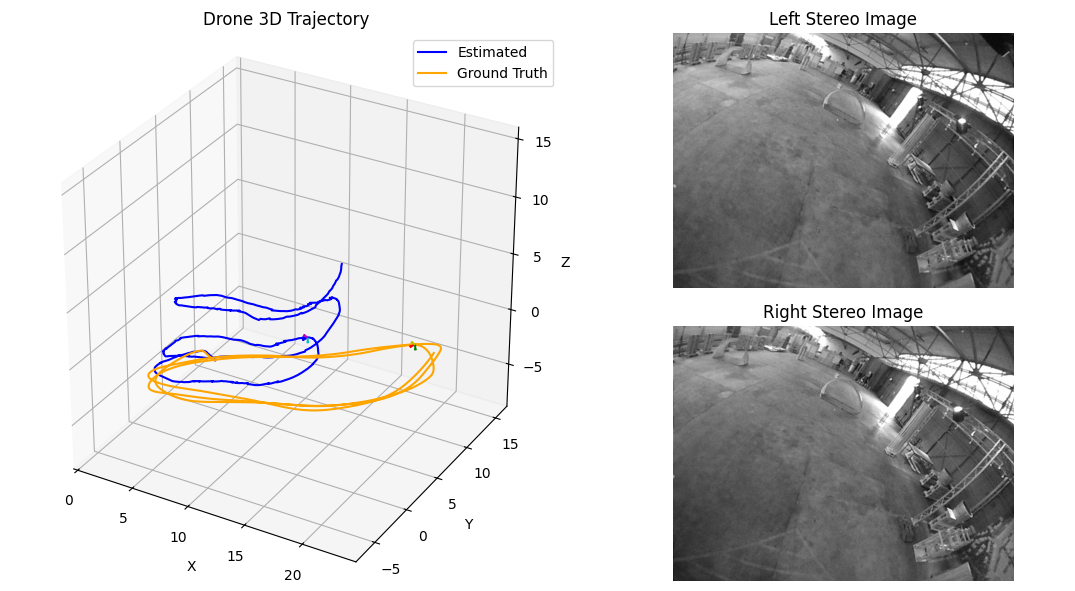
\includegraphics[width=0.8\linewidth]{figures/kf_validation_results.png}
    \caption{Kalman filter results on validation set with tracks from both estimated and ground truth performance.}
    \label{fig:kalman_results_validation_set}
\end{figure}

It is observed that the general shape of the movement is identified and supported in the x and y axes. However, there is significant observed drift in the z axes, as seen by the upward corkscrew movement of the drone as per the estimator. Ultimately, the filter was tuned to get an RMSE of [5.02, 3.17, 4.30] for the x, y and z axes respectively.

\end{document}